\chapter{Bausteine von Reactive Programming}\label{realisierung} 
Durch große Datenraten, Datenmengen und viele vernetzte Geräte und Dienste die zur heutigen Zeit in Umlauf sind, entstehen viele Informationen die verarbeitet werden können beziehungsweise müssen. Durch die vielen Berechnungen und Verarbeitungsschritte die dafür nötig sind, spielt hier das Gesetz von Amdahl eine große Rolle \cite{Amdahl.}. Dieses besagt, dass nie alle Teile eines Programms parallel ausgeführt werden können. Deshalb zerlegt man das Programm in eine sequentiellen und einen parallelen Teil. Reactive Programming versucht nun eine Lösung abzubilden, welche die Auslastung der Rechenressourcen optimiert und die Anzahl der Stellen welche serialisiert ablaufen zu verringern \cite{Boner.}. Ein Ansatz diese Lösung zu realisieren ist die Verwendung von besagten Reactive Streams. Neu auftretende Daten werden als Ströme betrachtet, die unter Beobachtung stehen und Änderungen sowie Bearbeitung der Daten asynchron und parallel zu den anderen Funktionen einer Anwendung ausgeführt werden können. Damit dieses Verfahren der Datenverarbeitung funktioniert, sind einige Konzepte zu beachten.
\section{Observer Pattern}
Ein bewährtes und klassisches Vorgehen bei Anwendungsanforderungen dieser Art ist das schon 1994 von Erich Gamma beschriebene Entwurfsmuster, dem \textit{Observer-Pattern} \cite{Gamma.2011}. Auch hier lässt sich wieder die GUI als Beispiel heran ziehen. Man betrachte man eine Oberfläche welche die Temperatur im Raum anzeigt. Um nun das Beobachtermuster zu implementieren, muss der sich ändernde Wert, der zum Beispiel von einem Temperatursensor gemessen wird, beobachtet werden. Dieser Sensor repräsentiert in Abbildung \ref{pic:observerpattern} eine Implementierung des Subject. Man nehme an auf der GUI soll der Temperaturwert als Balkendiagramm(BarChartForTemp), also als Art Thermometer dargestellt werden. Ebenso soll die aktuelle Temperatur in Schrift(LabelForTemp) auf der GUI erscheinen. Die beiden Objekte implementieren das Observer-Interface wie in Abbildung \ref{pic:observerpattern} gezeigt. Dies heißt wiederum, dass diese beiden Observer die \textit{register()}-Methode des Subjects aufrufen und somit in die Observer-Liste dieses Subjects, also dem Sensor, aufgenommen werden. Ändert sich nun zum Beispiel die Temperatur wird die \textit{notifyObservers()}-Methode aufgerufen, was heißt, dass über die Liste der Observer iteriert wird und die \textit{update()}-Methode jedes Observers aufgerufen wird.
\begin{figure}[hbt]
	\centering
	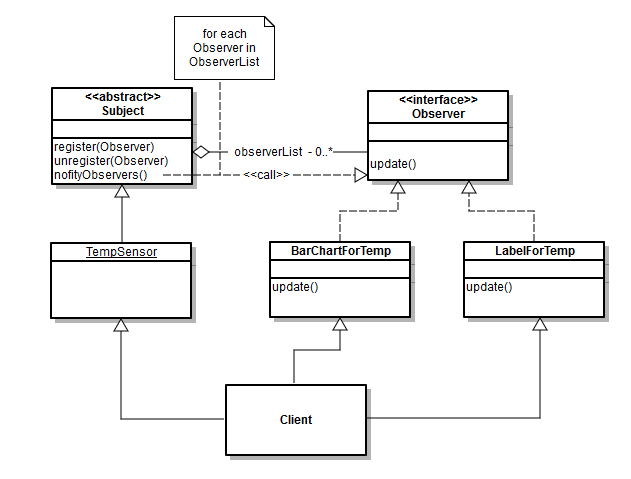
\includegraphics[width=0.85\textwidth]{Abb/observerpattern_self}
	\caption{Schematischer Aufbau eines Observer Patterns.}
	\label{pic:observerpattern}
\end{figure}
Diese Methoden können nach dem \textit{Push} oder \textit{Pull} Verfahren implementiert werden. Bei Verwendung des Push-Modells wird dem Observer der Wert des geänderten Parameters direkt mitgeteilt. Das Pull-Modell verfolgt den Ansatz, dass der Observer eine Information erhält, dass sich Werte geändert haben, er muss jedoch über die Getter-Methoden die für ihn relevanten Werte aktiv nachfragen. Je nach Vorgehen ergeben sich Vor- und Nachteile. Der Push-Ansatz steht eher für lose Kopplung, da der Observer keine Details des Subject kennen muss. Jedoch sinkt dadurch die Flexibilität, da Observer Interfaces exakter beschrieben werden müssen, damit das Subject weiß, welche Informationen weiter gereicht werden sollen. Die Kopplung im Vergleich zum Pull-Ansatz ist nicht wirklich lose, da jeder Beobachter wissen muss, welche Daten das observierte Objekt repräsentiert und wie auf diese Daten zugegriffen werden kann. Jedoch findet sich hier die Flexibilität wieder, da jeder Beobachter wenn er Information braucht, exakt diese Daten abrufen kann und sich nicht auf die korrekte Datenverteilung des Subjects verlassen muss.
\section{Reactive Streams}
Nach dem anfangs erwähnten Observer Pattern werden die Streams observiert und die Daten werden den Observern publiziert. Verfügen diese Observable Streams nun über die Funktionalität des Back Pressures ist eine nicht blockierende asynchrone Bearbeitung möglich. Nach diesen Voraussetzungen wurde in der Welt der JVM die Initiative der \textit{Reactive Streams} geschaffen, um einen Standard für diese Art von Verarbeitung zu etablieren \cite{rsmain}. Das zusätzlich zu bewältigende Problem ist die unterschiedliche Implementierung der bereits existierenden reaktiven Frameworks. Durch die Standardisierung soll eine Kompatibilität von reaktiven Komponenten untereinander gesichert werden, auch wenn besagte Komponenten auf unterschiedliche Frameworks basieren. Viele Entwicklerteams von reaktiven Frameworks haben sich mittlerweile dieser Initiative angeschlossen und die Schnittstellen soweit angepasst, dass diese Kompatibilität gewährleistet werden kann \cite{rslsting}. Mit Java 9 wird in der sogenannten \textit{Flow API} eine Implementierung nach den \textit{Reactive Streams} Kriterien geliefert \cite{flowdoc}. Ein Anwendungsbeispiel wird von der offiziellen Java-Community bereits zur Verfügung gestellt \cite{flowexmpl}. Da bereits eine Art von Streams seit Java 8 als API zur Verfügung stehen muss eine Abgrenzung zwischen diesen und den Reactive Streams verdeutlicht werden. Durch die ähnliche Art der Verwendung beider ist eine Verwechslung nicht ausgeschlossen, obwohl unterschiedliche Konzepte realisiert werden. Daher folgt eine kurze Beschreibung der Java 8 Streams und eine allgemeine Unterscheidung zu den im weiteren Lauf verwendeten Reactive Streams. 
\subsection{Java 8 Streams}
Das Konzept der Streams stellt eine Abstraktion für Folgen von Bearbeitungsschritten auf Daten dar \cite{Inden.2015}. Streams erinnern an Collections, sind jedoch nur einmal traversierbar und nehmen keine direkten Speicherung der Daten vor. Collections können auch als Streams repräsentiert werden. Nahe liegt die verbreitete Analogie der Fließbandverarbeitung. Man hat eine Menge von Objekten die nacheinander gewissen Arbeitsschritten unterzogen werden. Diese werden einmalig durchgeführt und die Zwischenergebnisse bleiben nicht vorhanden. In Listing \ref{lst:streamsandbulk} sieht man, dass mit dem Methodenaufruf \textit{stream()} auf der Collection ein Stream parametrisiert auf den selben Datentyp wie die Collection erstellt werden kann. Es findet keine Änderung an den einzelnen Elemente statt, denn es wird nur das Ergebnis der Operation ausgegeben.
\lstinputlisting[linerange={7-14}, float=hbt, caption={Beispiel Erstellung, Verarbeitung und Ergebnisermittlung von Streams.}, label=lst:streamsandbulk]{../SystemMonitor/examples/streamsandbulk/StreamsAndBulk.java}
\subsubsection{Bulk Operations}
Bulk Operations gelten als funktional und sind seit Java 8 auf Collections sowie Streams anwendbar. Diese Operationen müssen nicht separat implementiert werden und können direkt auf Collections oder Streams ausgeführt werden. Jedoch sind nicht zu beiden Arten die exakt gleichen Operation verfügbar. Somit kann durch eine Operation zum Beispiel eine Veränderung an jedem Objekt einer Liste ausgeführt werden, oder eben auf jedem Objekt welches einen Stream durchquert. Die Operation können verkettet werden. Als Ergebnis werden die Elemente, zum Beispiel nach der Filterung ausgegeben, oder in einer neuen Liste gespeichert. Auch bei einer Verkettung wird immer nur das Ergebnis weiter gereicht, die Eingangswerte bleiben unverändert. Erwähnung sollten noch die unterschiedlichen Arten von Operationen finden. Man unterscheidet zwischen drei Arten: \textit{Erzeugung}, \textit{Berechnung} und \textit{Ergebnisermittlung} die sich wie folgt abbilden lassen \cite{Inden.2015} : 
\begin{displaymath}
\underbrace{Quelle \Rightarrow STREAM}_{Erstellung} \Rightarrow \underbrace{OP_{1} \Rightarrow OP_{2} \Rightarrow ... \Rightarrow OP_{n}}_{Berechnung} \Rightarrow \underbrace{Ergebnis}_{Ergebnisermittlung}
\end{displaymath}
Bei der Erzeugung wird von der Änderung der Datenrepräsentation von einem Datentyp einer Collection oder eines Arrays in einen Stream gesprochen. Java bietet hier für jeweils Arrays oder Collections Methoden an. Resultierend erhält man einen Stream. Eine Reihe von Berechnungen kann nun verkettet stattfinden, zum Beispiel eine Transformation oder Filterung nach Kriterien. Sind die Operationen abgeschlossen wird das Ergebnis, zum Beispiel auf der Konsole, ausgegeben oder in einem Datentyp gespeichert. Konkret ist der Ablauf in Listing \ref{lst:streamsandbulk} zu sehen. Wie vorhin schon erwähnt wird via Methodenaufruf eine Stream-Repräsentation der Collection geschaffen. Die Berechnung beziehungsweise Bearbeitung findet in der Konkatenation der Operation \textit{map()} und \textit{filter()} statt. Zuerst wird jeder String in Großbuchstaben transformiert, und das Ergebnis an die Filter-Operation weitergegeben. Anschließend wird gefiltert ob der String den angegeben Kriterien genügt. Die Ergebnisermittlung findet in der \textit{forEach()}-Methode statt, da hier jedes Element, das nach dem filtern noch übrig ist, auf die Konsole geschrieben wird. Es können beliebig viele Stream-Objekte von einer Collection erstellt werden, jedoch ist die Traversierung, und somit die Verwendung, eines Streams nur einmalig möglich.
\subsection{Unterscheidung zu Reactive Streams}
Die vorab beschriebenen Streams und die dazugehörigen Operationen funktionieren durch die Verwendung des Pull-Verfahrens. Mittels Iterator wird immer ein weiteres Element von der Datenquelle geholt und darauf die Operationen angewandt. Diese Streams sind nur einmalig verwendbar. Wird von Reactive Streams gesprochen gelten diese Eigenschaften nicht. Es wird nach dem Push-Verfahren gehandelt, was heißt, das nicht mit dem Iterator gearbeitet wird. Auch müssen diese Streams nicht endlich sein, was wiederum heißt, dass die Anzahl der Elemente nicht vorab bekannt sein muss. Zusätzlich ist eine mehrfache Verwendung dieser Reactive Streams möglich. Die Bulk Operations sind auch auf Reactive Streams möglich, es liegen jedoch viele weitere Operationen vor die speziell für die Verwendung des Push-Verfahrens implementiert wurden. Diese signifikanten Unterschiede zeigen, dass wenn auch in beiden Fällen von Datenströmen gesprochen wird, der grundlegende Gedanke wie mit Streams umgegangen wird ein anderer ist.
\section{Back Pressure}
Der weitere wichtige Aspekt der Reactive Streams ist die bereits erwähnte Eigenschaft des nicht blockierenden Back Pressures. Man betrachtet hier den Push-Ansatz. Ein Producer generiert Daten, die ein Consumer verarbeitet. Es kann nun passieren das mehr Daten produziert werden als konsumiert werden können. Wird darauf nicht reagiert, kann es zu starken Ressourcenproblemen oder zu einem Programmabsturz durch einen \textit{OutOfMemoryError} kommen. Um dies zu verhindern, benötigt man eine Möglichkeit, die Anzahl der zu verarbeitenden Objekte zu regulieren. Ein sogenannter \textit{Feedback Channel} steht dafür zur Verfügung. Über diesen kann ein Consumer seinem Producer mitteilen, mit wie vielen Objekten er maximal umgehen kann. Dadurch ergibt sich die Möglichkeit auf Seiten des Producers seine Datenbeschaffung und Datenweitergabe zu regulieren, sodass der Producer zu jeder Zeit verwendbar bleibt und nicht blockiert. Dies geschieht zum Beispiel über einen zusätzlichen Puffer an Ausgang des Producers, wodurch die direkte Datenweitergabe verzögert werden kann. Dies besteht jedoch nur, wenn es dem Producer auch möglich ist, seine Geschwindigkeit zu steuern. Zu beachten ist, dass grundsätzlich jeder Consumer über einen Eingangspuffer verfügt, in welchem die geforderten Objekte zwischen lagern. Wird der Back Pressure nicht richtig behandelt oder die Puffer fehlerhaft konfiguriert, kann es zu eine \textit{MissingBackPressureException} kommen.
